\documentclass[a4paper,10pt,french]{scrartcl}

\usepackage{background}

\usepackage{fontspec}
\usepackage{babel}

\usepackage{siunitx}

\usepackage{libertine}

\usepackage{import}
\usepackage{transparent}

\usepackage[
  automark,
  autooneside=false,% <- needed if you want to use \leftmark and \rightmark in a onesided document
  % IF Head linewidth
  % headsepline
]{scrlayer-scrpage}

\usepackage{hyperref}
\hypersetup{
    colorlinks,
    citecolor=black,
    filecolor=black,
    linkcolor=black,
    urlcolor=blue
}

\pagestyle{scrheadings}
\clearpairofpagestyles

\graphicspath{{./assets/}}

\newcommand{\incfig}[2][1]{%
    \def\svgwidth{#1\columnwidth}
    \import{./figures/}{#2.pdf_tex}
}


%--------------------------------------------|
\DeclareSIUnit{\reactif}{R}
\DeclareSIUnit{\VAR}{\volt\ampere\reactif} 
%--------------------------------------------|



% ? color boxs ---------------------------------------------------------------|

\usepackage[most]{tcolorbox}


%? Basic environnement with a title and a principal color

\renewenvironment{colorbox}[2]
  {
    \begin{tcolorbox}[colback=#2!5!white,colframe=#2!50!black,title=#1]
  }
{
  \end{tcolorbox}
  }
  

% Environement definition with "Definition : #title", color green

\newenvironment{definition}[1]
  { \begin{colorbox}{Définiton : #1}{green} } { \end{colorbox} }

  \newenvironment{definition*}[0]
  { \begin{colorbox}{Définiton}{green} } { \end{colorbox} }


% Environement exemple with "Exemple : #title", colr gray

\newenvironment{exemple}[1]
{ \begin{colorbox}{Exemple : #1}{gray} } { \end{colorbox} }

\newenvironment{exemple*}[0]
{ \begin{colorbox}{Exemple}{gray} } { \end{colorbox} }


%? Environement attention with a title, color red

\newenvironment{attention}[1]
{ \begin{colorbox}{#1}{red} } { \end{colorbox} }
% ? --------------------------------------------------------------------------|

%$ Vertically Align

\newenvironment{vertAlign}{\null\vfill}{\vfill\null}


\newcommand{\universityLogo}{
	\backgroundsetup{contents=\centering 
\includegraphics{logo.png}, scale=0.65, angle=0, placement=top, hshift=12cm, vshift=0, opacity=1}
}

\input{ressources/informations.tex}

% \backgroundsetup{contents=
\includegraphics{assets/logo.png}, scale=0.35, angle=0, placement=top, hshift=25cm, vshift=-0.8cm, opacity=1}

\backgroundsetup{contents=\includegraphics{example-image-a}, scale=0.35, angle=0, placement=top, hshift=25cm, vshift=-0.8cm, opacity=1}

\setkeys{Gin}{width=7.5cm}

% IF right head title wanted
% \ohead{\rightmark}
\cfoot{{\usekomafont{pagenumber}\large - \thepage\ -}}

\usepackage{lipsum}

% ! additionals packages ----------┐
% \usepackage{pdfpages}          %!|
% \usepackage{csvsimple}         %!|
% \usepackage{tikz}              %!|
% \usepackage{pgfplots}          %!|
% \usepackage{circuitikz}        %!|
% \usepackage{subcaption}        %!|
% \usepackage{setspace}          %!|
% \usepackage{amsmath}           %!|
%!                             %! /
%!                            %! /
\usepackage{pifont} %\ding{51} %!|
\usepackage{enumitem}          %!|
\usepackage{multicol}          %!|
\usepackage{listings}          %!|
%!                            %! \
%!                             %! \
%!                                 |
%! --------------------------------┘

% $ codeStyle -------------------------------┐
%New colors defined below
\definecolor{codegreen}{rgb}{0,0.6,0}
\definecolor{codegray}{rgb}{0.5,0.5,0.5}
\definecolor{codepurple}{rgb}{0.502,0.502,0.0}
\definecolor{backcolour}{rgb}{0.95,0.95,0.95}

\lstdefinelanguage{ST}
{
	morekeywords={
	case,of,if,then,end_if,end_case,super,function_block,extends,var,
	constant, byte,,end_var,var_input, real,bool,var_output,
	dint,udint,word,dword,array, of,uint,not,adr, program, for, end_for, while, do, end_while, repeat, end_repeat, until, to, by, else, elsif, var_in_out
	},
	otherkeywords={
		:, :=, <>,;,\,.,\[,\],\^,1,2,3,4,5,6,7,8,9,0,TRUE, FALSE, \{attribute,  \'hide\'\}
	},
	keywords=[1]{
		case,of,if,then,end_if,end_case,super,function_block,extends,var,
		constant, byte,,end_var,var_input, real,bool,var_output,
		dint,udint,word,dword,array, of,uint,not,adr, :, :=, <>,;,\,.,\[,\],\^,program, for, end_for, while, do, end_while, repeat, end_repeat, until, to, by, else, elsif, var_in_out
	},
	keywordstyle=[1]\color{blue},
	keywords=[2]{
		1,2,3,4,5,6,7,8,9,0, TRUE, FALSE
	},
	keywordstyle=[2]\color{codepurple},
	keywords=[3]{
		\{attribute,  \'hide\'\}
	},
	keywordstyle=[3]\color{codegray},
	sensitive=false,
	morecomment=[l]{//}, 
	morecomment=[s]{(*}{*)},
	morestring=[b]{"},
	morestring=[b]{'}
}

\lstset{
	language={ST},
	backgroundcolor=\color{backcolour},
	commentstyle=\color{codegreen}\textit,
	keywordstyle=\color{blue},
	numberstyle=\tiny\color{codegray},
	stringstyle=\color{codepurple},
	basicstyle=\ttfamily\scriptsize,
	breakatwhitespace=false,         
	breaklines=true,                 
	captionpos=b,                    
	keepspaces=true,                 
	numbers=left,                    
	numbersep=5pt,                  
	showspaces=false,                
	showstringspaces=false,
	showtabs=false,                  
	tabsize=2
}
          %$ |
\setmonofont{JetBrainsMono}[
  Contextuals={Alternate},
  Path=./ressources/fonts/JetBrains_Mono/,
  Extension = .ttf,
  UprightFont=*-Regular,
  BoldFont=*-Bold,
  ItalicFont=*-Italic,
  BoldItalicFont=*-BoldItalic
]

\lstdefinelanguage{algorythme}
{
	morekeywords={
    Pour, pour, allant, Allant, Si, si, Alors, alors, Sinon, sinon,
    ecrire, Ecrire, Écrire, écrire, Algo, Algorythme, algo, 
    algorythme, Début, Debut, debut, Fin, FIN, DEBUT
	},
	otherkeywords={
		:, =, <>,;,/
	},
  keywords=[1]{
    Algo, Algorythme, algo, algorythme
  },
  keywordstyle=[1]{
    \bfseries\color{red!75}
  },
	keywords=[2]{
    Pour, pour, allant, Allant, Si, si, Alors, alors, Sinon, sinon, 
    Selon, selon 
	},
	keywordstyle=[2]\color{blue!75},
 keywords=[3]{
  ecrire, Ecrire, Écrire, écrire
 },
 keywordstyle=[3]{
  \color{green!50!black}
 },
 keywords=[4]{
  Début, Debut, debut, DEBUT, Fin, FIN
 },
	sensitive=true,
	morecomment=[l]{//}, 
	morestring=[b]{"},
	morestring=[b]{'},
  literate=
      {<-}{$\leftarrow$}{1}%
      {->}{$\rightarrow$}{1}%
      {<=}{$\leq$}{1}%
      {=<}{$\leq$}{1}%
      {=>}{$\geq$}{1}%
      {>=}{$\geq$}{1}%
      {--}{{{\color{blue}——}}}{1}}


\lstset{
	language={algorythme},
	backgroundcolor=\color{backcolour},
	commentstyle=\color{codegreen}\textit,
	keywordstyle=\color{blue},
	numberstyle=\tiny\color{codegray},
	stringstyle=\color{codepurple},
  basicstyle=\footnotesize\ttfamily,
	breakatwhitespace=false,         
	breaklines=true,                 
	captionpos=b,                    
	keepspaces=true,                 
	numbers=left,                    
	numbersep=5pt,                  
	showspaces=false,                
	showstringspaces=false,
	showtabs=false,                  
	tabsize=2
}


\newcommand{\algorythme}[1]{
        \lstinputlisting[style=algorythme]{#1}
    }  %$ |
%$ ------------------------------------------┘


\setcounter{tocdepth}{5}
% \renewcommand\thesection{\arabic{section}}

% ----------------------------------------------------------------------|
\begin{document}


  \titlehead{{\Large Mathématiques} \hfill 1$^{st}$ year - 2022/2023}
  \title{How it's look like ? (Title)}
  \author{\firstName\ \lastName \\Group \groupNumber}
  \date{\today}
  \publishers{\university}

  \maketitle

  \noindent\makebox[\linewidth]{\rule{7.5cm}{0.4pt}}

  \tableofcontents
  \newpage

  % ! begin here

  \section{Specifications}

    \begin{vertAlign}
      \begin{itemize}[label=\color{green}\ding{51}]

        \Large
        \setlength\itemsep{0.8cm}


        \item The living room lighting is activated if a person is detected in the room and if the brightness is insufficient (\textbf{less than 100 lux}).

        \item The lighting of the office (located in the bedroom) is realised from \textbf{2 push buttons}.

        \item The control of the roller shutter in the living room is achieved by means of \textbf{2 push buttons "Up" and "Down"}.

        \item A space heater connected to a bedroom socket can be switched off by a \textbf{push button}.

        \item If the humidity is too high (\textbf{over 70 \%}), the ventilation system will be activated.

        \item[\color{red}\ding{56}] {\color{gray}\textit{BONUS -}} Mathématiques of a \textbf{generalized and simultaneous extinction} of the lighting circuits.
      \end{itemize}
    \end{vertAlign}

  
  \newpage

  \section{Answers examples}

    \subsection{Colorbox examples}

      \begin{colorbox}{{$y=Ce^{kx}$}}{gray}
            
        \begin{quote}
          For the function $y=Ce^{kx}$ to be linear, It is necessary \textbf{to apply the function \color{red}$g(x)=\ln(x)$}
          
          \vspace{0.5cm}

          $a_0=\ln(C)$

          $a_1=k$

          \begin{eqnarray*}
            g(x) &=& a_0 + a_1 x \\
                 &=& \ln(C) + kx \\
          \end{eqnarray*}

          \vspace{0.5cm}

          There is a restriction on the values that can be taken by $C$, $k$ and $x$ to be allowed to apply this linking method. Indeed, the function $\ln(x)$ is defined on $]0:+\infty[$

        \end{quote}
      \end{colorbox}

      \begin{colorbox}{}{green}
       \textit{Colorbox without title} 

       \vspace{0.5cm}

       \lipsum[10]
      \end{colorbox}

      \newpage

      \subsubsection{Definition color block}
      \noindent \begin{definition}{Speed controller}
        The speed at which the cylinder rod exits is determined by the speed at which the air is vented from the exhaust chamber. This speed is determined by the adjustable restriction on the exhaust line.


        \begin{multicols}{2}
          
          \begin{vertAlign}
            \centering \textit{The flow rate should be adjusted as close as possible to the cylinder}
          \end{vertAlign}

          \begin{vertAlign}
            \centering 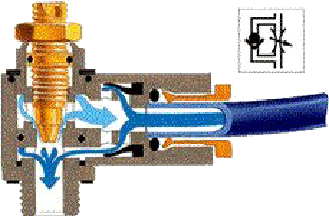
\includegraphics[width=5cm]{assets/auxiVitesse.png}
          \end{vertAlign}
        \end{multicols}
      \end{definition}
      \noindent \begin{definition*}{Pythagorean Theorem \textit{Environement without argument but with "Definition" by default}}
       
        \begin{multicols}{2}
          
          \begin{vertAlign}
            If a triangle is right-angled, the square of the length of the hypotenuse (or side opposite the right angle) is equal to the sum of the squares of the lengths of the other two sides.

            \begin{equation*}
              c=\sqrt{a^2+b^2}
            \end{equation*}
          \end{vertAlign}

          \columnbreak

          \begin{vertAlign}
            \centering 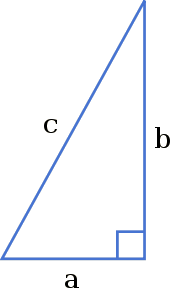
\includegraphics[width=2cm]{assets/pythagoreanTheorem.png}
          \end{vertAlign}
        \end{multicols}
      \end{definition*}

      \begin{colorbox}{}{green}
        
        \lipsum[2]{1}
      \end{colorbox}

      \newpage
      \subsubsection{Example color block}

        \noindent \begin{exemple}{Program in ST language}
          \lstinputlisting[language=ST]{assets/StExample.txt}
        \end{exemple}

        \paragraph*{Program in ST language}
        \noindent \begin{exemple*}
          \lstinputlisting[language=ST]{assets/StExample.txt}
        \end{exemple*}

        \begin{colorbox}{}{green}
          \lstinputlisting[language=algorythme, backgroundcolor=\color{green!5!white}]{assets/algoExample.txt}
        \end{colorbox}

  \section{Second section}

    \subsection{blabla}
    \subsection{blablabla}

  \section{Conclusion}
\end{document}